\section{Every run: per-seed results and full learning curves}\label{app:results}

This appendix reports every final run.
\Cref{tab:seeds} gives the last-checkpoint divergence and success of each seed, including every run that does not meet the operational thresholds.
\Cref{fig:curves-first} and the following figures show the full learning curves of every core cell, drawn by \texttt{scripts/analyze.py} from the evaluation records: $f$-PG against learner transitions (left), \ERFB{} and \DMFB{} against FB pretraining updates (middle), and the 300 \DMFB{} latent steps at the final FB snapshot (right); thin lines are seeds and thick lines means.
A run marked ``not reached'' in \cref{tab:convergence} did not meet the thresholds at any assessed checkpoint within the budget: every evaluated checkpoint for $f$-PG, and every FB snapshot after completed adaptation for \ERFB{} and \DMFB{} (for \DMFB, the latent after its 300 steps). The intermediate \DMFB{} iterates evaluated at the final snapshot (right-hand panels) are not assessed by this rule; in \vn{s11.dm.mid_cross}{three} runs they entered the threshold region and left it before the final step (\cref{sec:results-finite}).

{\footnotesize\setlength{\tabcolsep}{4pt}
% GENERATED by report/verify/make_tables.py from the saved run files (runs/jobs/*).
% Every completed run: final held-out JS and success per seed (core and compact ablations).
% Do not edit by hand: rerun  python3 report/verify/verify_results.py

\begin{longtable}{@{}lllccccccl@{}}
\caption{Every final run: held-out divergence (nats) and success at the last checkpoint for each seed, and the seeds that meet the operational thresholds there (JS $\le0.10$ and success $\ge0.80$). Finite values are exact; continuous values are Monte Carlo estimates (500 rollouts).}\label{tab:seeds}\\
\toprule
maze & goal & method & JS s0 & JS s1 & JS s2 & succ.\ s0 & succ.\ s1 & succ.\ s2 & met\\
\midrule\endfirsthead
\toprule
maze & goal & method & JS s0 & JS s1 & JS s2 & succ.\ s0 & succ.\ s1 & succ.\ s2 & met\\
\midrule\endhead
\bottomrule\endfoot
finite open & (5,1) & \fPG{} (JS) & 0.001 & 0.003 & 0.026 & 1.000 & 0.999 & 1.000 & s0, s1, s2\\
 &  & \DMFB & 0.490 & 0.630 & 0.485 & 0.147 & 0.042 & 0.466 & none\\
 &  & \ERFB & 0.423 & 0.448 & 0.440 & 0.952 & 0.721 & 0.932 & none\\
\addlinespace
finite open & (5,5) & \fPG{} (JS) & 0.020 & 0.004 & 0.032 & 1.000 & 1.000 & 1.000 & s0, s1, s2\\
 &  & \DMFB & 0.489 & 0.484 & 0.398 & 0.529 & 0.453 & 0.368 & none\\
 &  & \ERFB & 0.272 & 0.374 & 0.230 & 0.999 & 0.978 & 0.999 & none\\
\addlinespace
finite open & (1,5) & \fPG{} (JS) & 0.002 & 0.002 & 0.004 & 0.999 & 1.000 & 1.000 & s0, s1, s2\\
 &  & \DMFB & 0.450 & 0.618 & 0.122 & 0.291 & 0.057 & 0.975 & none\\
 &  & \ERFB & 0.497 & 0.423 & 0.097 & 0.471 & 0.954 & 1.000 & s2\\
\addlinespace
finite four rooms & (5,1) & \fPG{} (JS) & 0.001 & 0.002 & 0.002 & 1.000 & 0.999 & 1.000 & s0, s1, s2\\
 &  & \DMFB & 0.645 & 0.559 & 0.562 & 0.058 & 0.068 & 0.136 & none\\
 &  & \ERFB & 0.427 & 0.448 & 0.435 & 0.926 & 0.932 & 0.976 & none\\
\addlinespace
finite four rooms & (5,5) & \fPG{} (JS) & 0.012 & 0.021 & 0.012 & 1.000 & 1.000 & 1.000 & s0, s1, s2\\
 &  & \DMFB & 0.244 & 0.554 & 0.629 & 0.950 & 0.031 & 0.001 & none\\
 &  & \ERFB & 0.226 & 0.435 & 0.382 & 0.998 & 0.651 & 0.668 & none\\
\addlinespace
finite four rooms & (1,5) & \fPG{} (JS) & 0.004 & 0.003 & 0.013 & 1.000 & 0.999 & 0.998 & s0, s1, s2\\
 &  & \DMFB & 0.198 & 0.622 & 0.275 & 0.971 & 0.048 & 0.865 & none\\
 &  & \ERFB & 0.079 & 0.321 & 0.434 & 0.994 & 0.986 & 0.828 & s0\\
\addlinespace
continuous & (5,1) & \fPG{} (JS) & 0.242 & 0.267 & 0.300 & 0.986 & 0.974 & 0.982 & none\\
 &  & \DMFB & 0.644 & 0.355 & 0.542 & 0.002 & 0.884 & 0.174 & none\\
 &  & \ERFB & 0.484 & 0.500 & 0.523 & 0.868 & 0.934 & 0.612 & none\\
 &  & expert & 0.0008 & 0.0009 & 0.0008 & 1.000 & 1.000 & 1.000 & s0, s1, s2\\
\addlinespace
continuous & (5,5) & \fPG{} (JS) & 0.359 & 0.414 & 0.340 & 0.974 & 0.922 & 0.962 & none\\
 &  & \DMFB & 0.555 & 0.548 & 0.352 & 0.584 & 0.004 & 0.834 & none\\
 &  & \ERFB & 0.659 & 0.549 & 0.515 & 0.434 & 0.122 & 0.260 & none\\
 &  & expert & 0.0007 & 0.0013 & 0.0010 & 1.000 & 1.000 & 1.000 & s0, s1, s2\\
\addlinespace
continuous & (1,5) & \fPG{} (JS) & 0.271 & 0.313 & 0.322 & 0.982 & 0.974 & 0.982 & none\\
 &  & \DMFB & 0.371 & 0.594 & 0.693 & 0.588 & 0.072 & 0.000 & none\\
 &  & \ERFB & 0.499 & 0.548 & 0.479 & 0.974 & 0.118 & 0.994 & none\\
 &  & expert & 0.0008 & 0.0008 & 0.0005 & 1.000 & 1.000 & 1.000 & s0, s1, s2\\
\addlinespace
ablation, four rooms & (5,5) & \fPG{} ($\KL(d\Vert q)$) & 0.010 & 0.017 & 0.009 & 1.000 & 1.000 & 0.998 & s0, s1, s2\\
 &  & \fPG{} ($\KL(q\Vert d)$) & 0.057 & 0.071 & 0.055 & 0.995 & 0.998 & 1.000 & s0, s1, s2\\
 &  & \ERFB, no orth. & 0.308 & 0.387 & 0.380 & 0.964 & 0.982 & 0.949 & none\\
 &  & \DMFB, no orth. & 0.389 & 0.502 & 0.508 & 0.605 & 0.392 & 0.433 & none\\
\addlinespace
\end{longtable}

}

\begin{figure}[p]
\centering
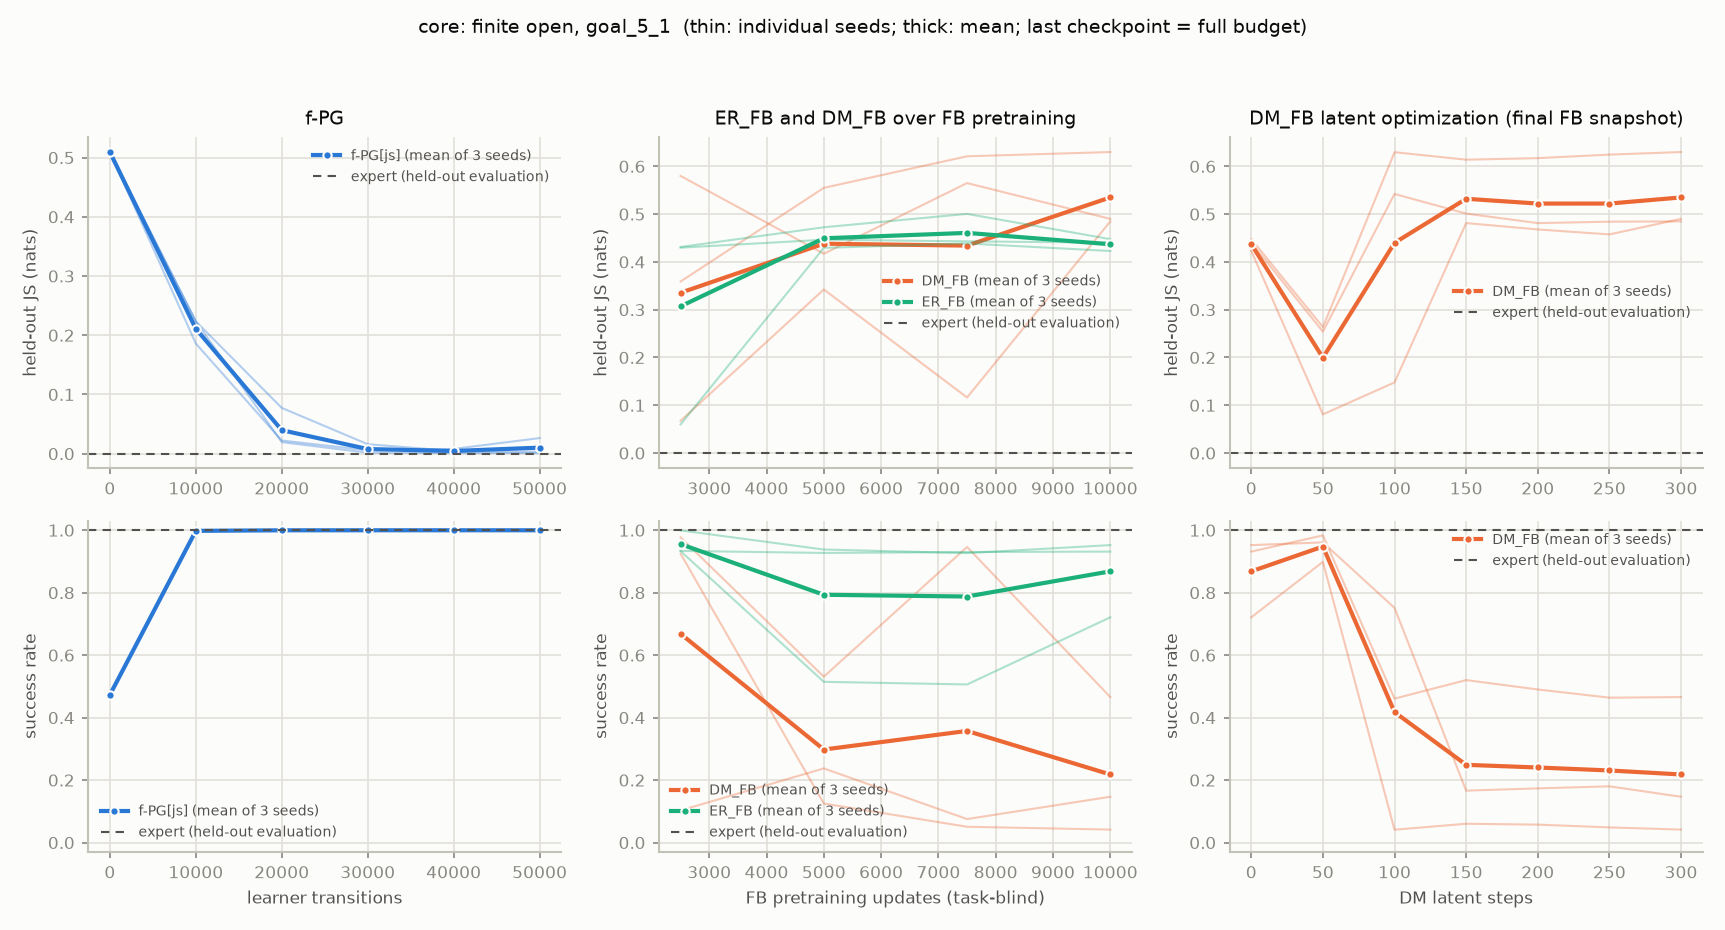
\includegraphics[width=\textwidth]{figures/curves_core_finite_open_goal_5_1.png}
\caption{Learning curves, core suite, finite open maze, goal (5,1).}\label{fig:curves-first}
\end{figure}

\begin{figure}[p]
\centering
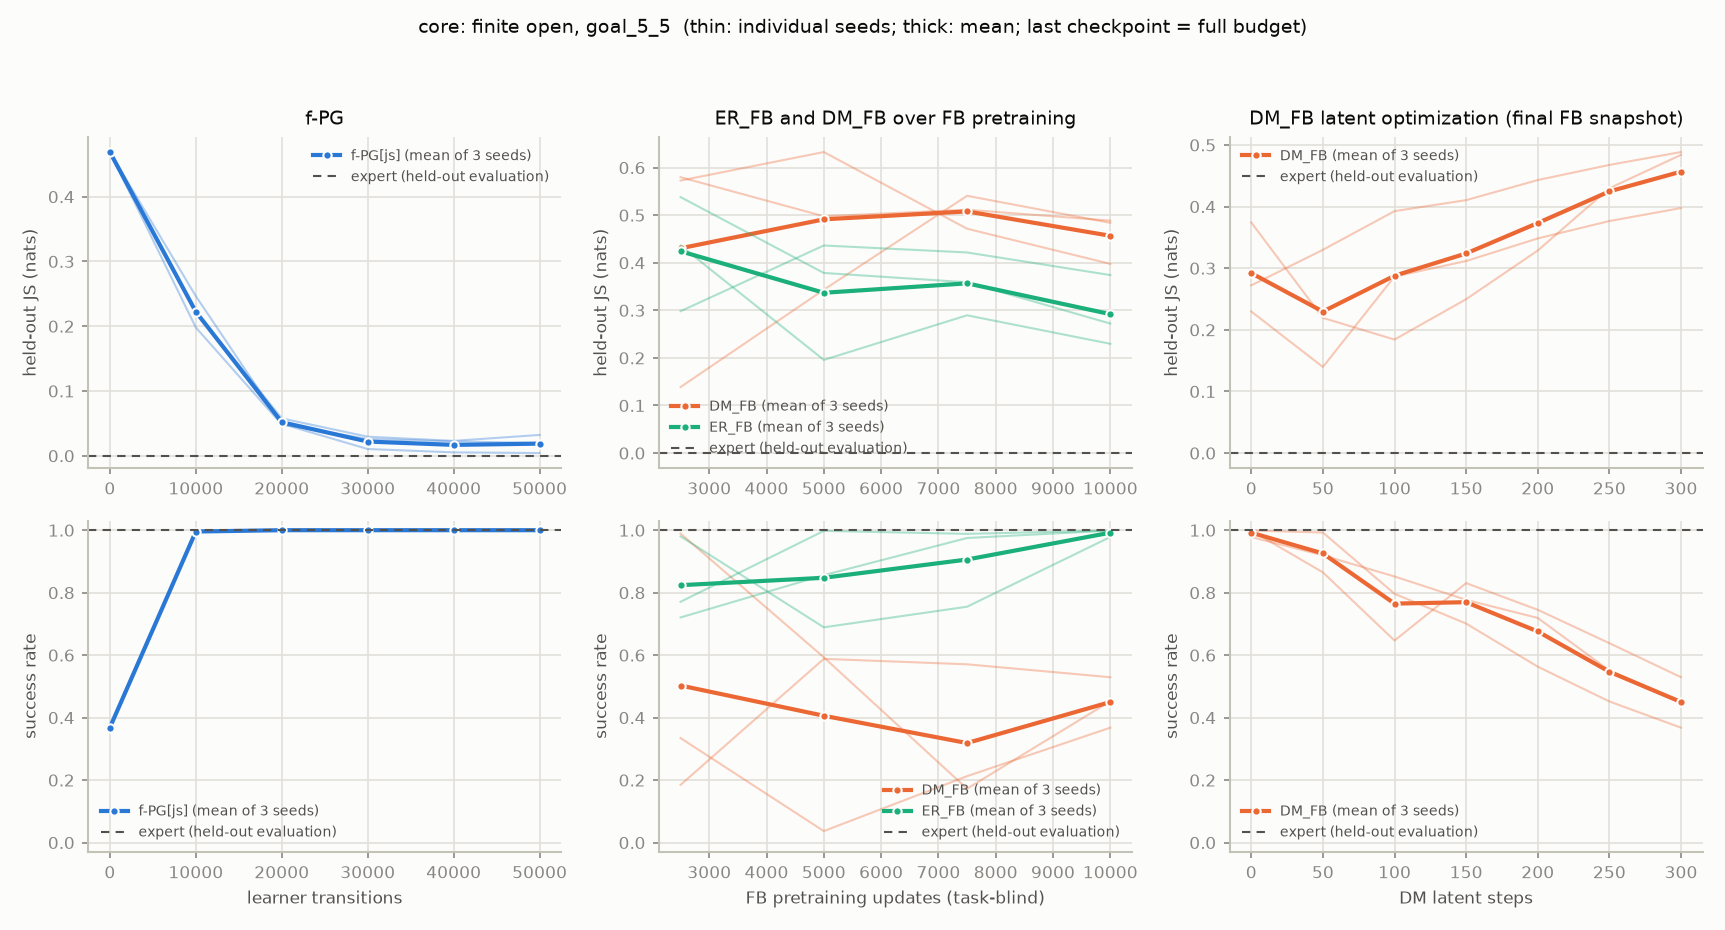
\includegraphics[width=\textwidth]{figures/curves_core_finite_open_goal_5_5.png}
\caption{Learning curves, core suite, finite open maze, goal (5,5).}
\end{figure}

\begin{figure}[p]
\centering
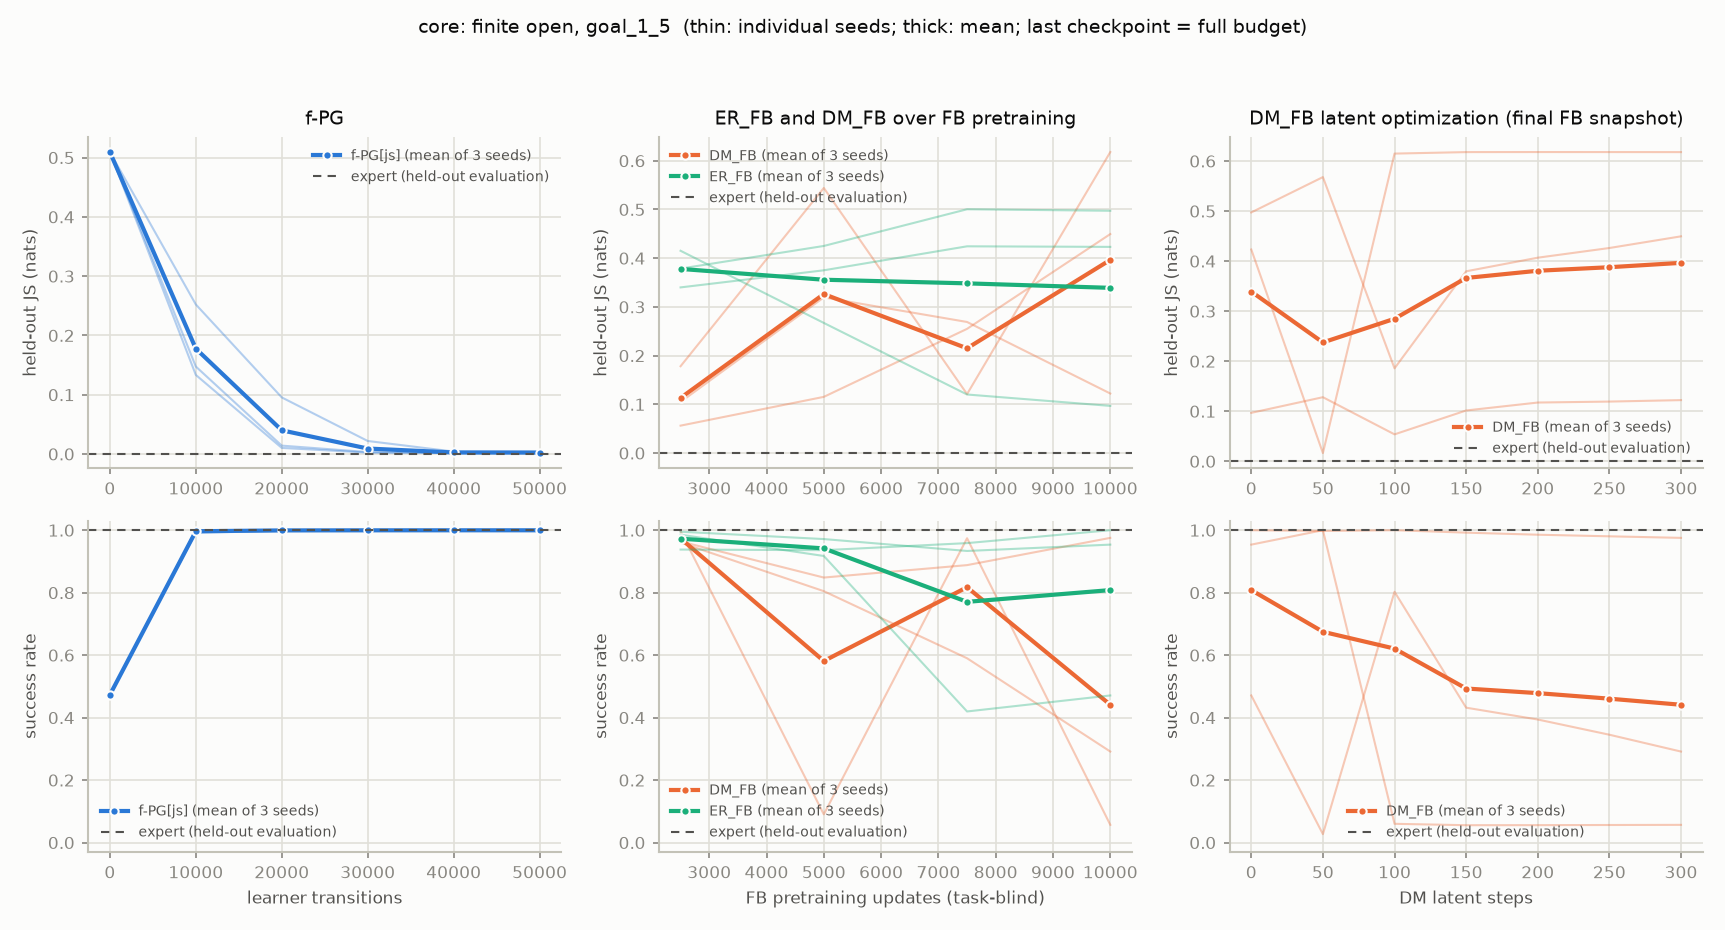
\includegraphics[width=\textwidth]{figures/curves_core_finite_open_goal_1_5.png}
\caption{Learning curves, core suite, finite open maze, goal (1,5).}
\end{figure}

\begin{figure}[p]
\centering
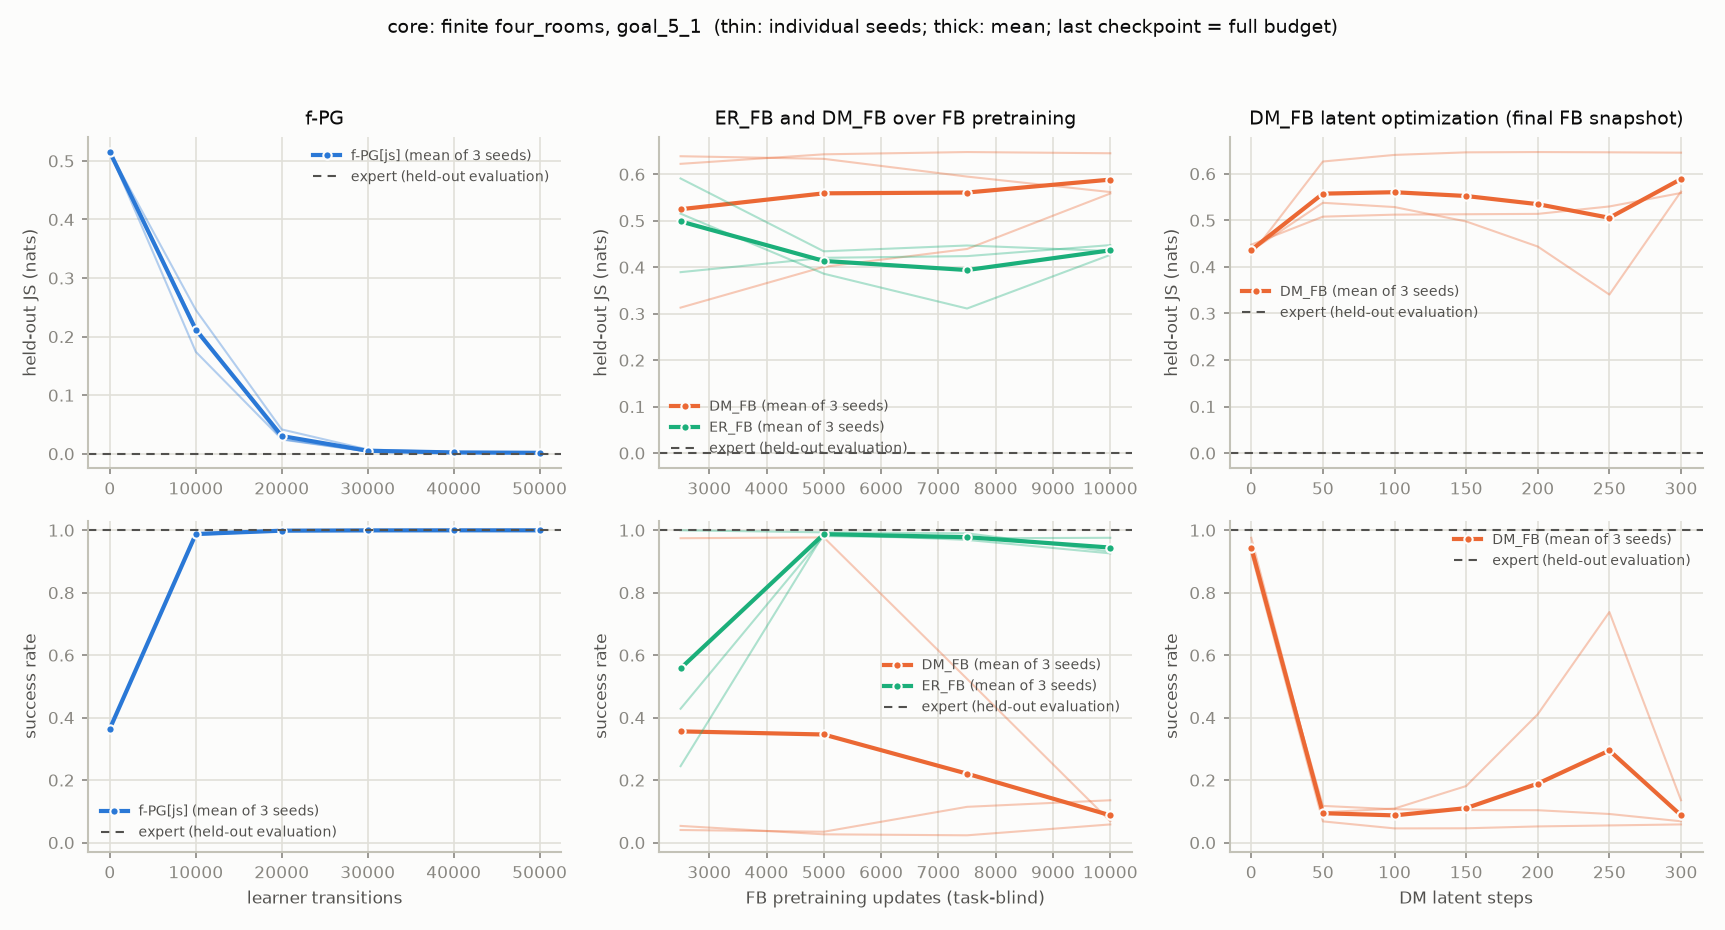
\includegraphics[width=\textwidth]{figures/curves_core_finite_four_rooms_goal_5_1.png}
\caption{Learning curves, core suite, finite four-rooms maze, goal (5,1).}
\end{figure}

\begin{figure}[p]
\centering
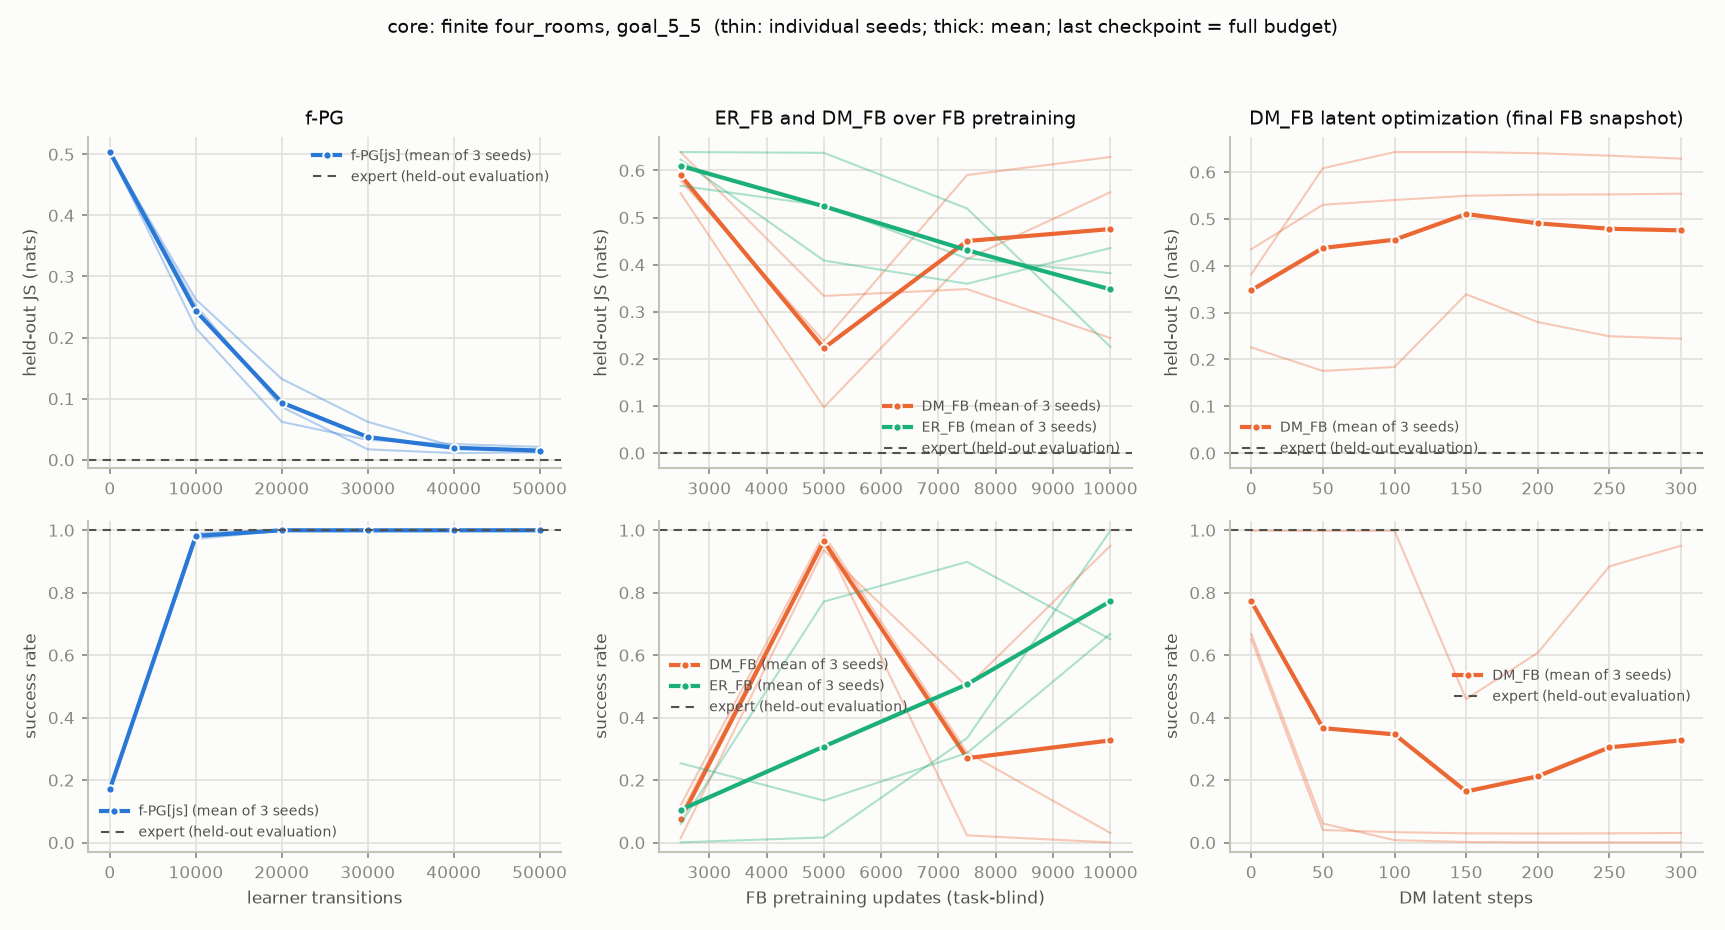
\includegraphics[width=\textwidth]{figures/curves_core_finite_four_rooms_goal_5_5.png}
\caption{Learning curves, core suite, finite four-rooms maze, goal (5,5).}
\end{figure}

\begin{figure}[p]
\centering
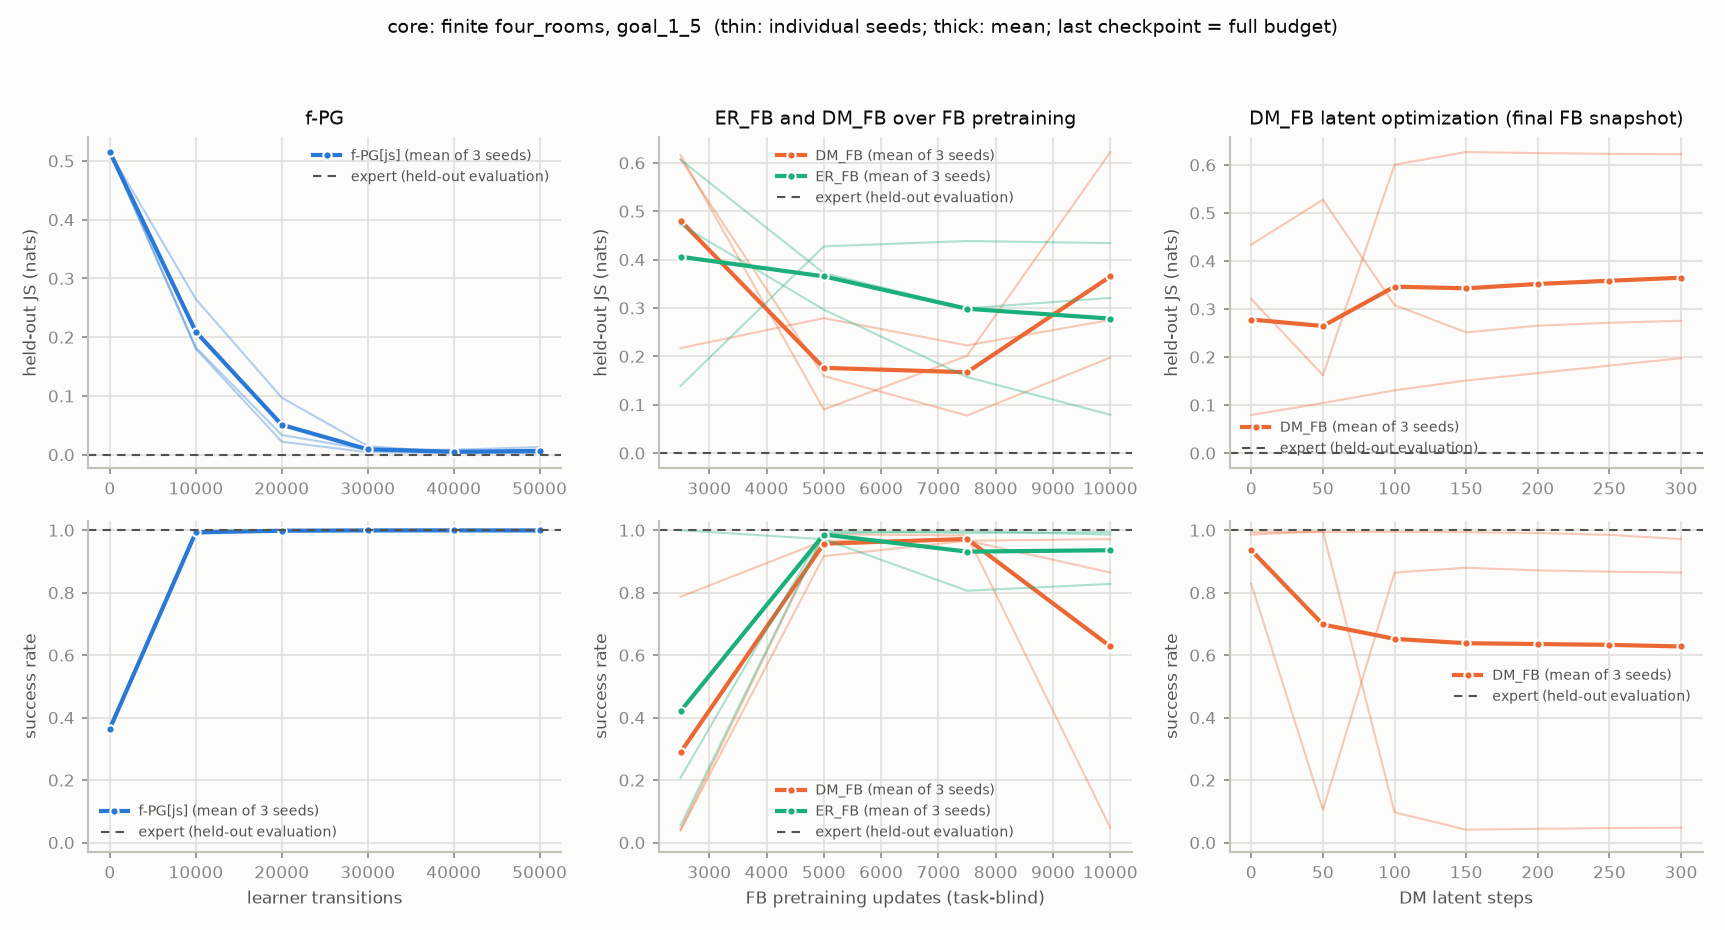
\includegraphics[width=\textwidth]{figures/curves_core_finite_four_rooms_goal_1_5.png}
\caption{Learning curves, core suite, finite four-rooms maze, goal (1,5).}
\end{figure}

\begin{figure}[p]
\centering
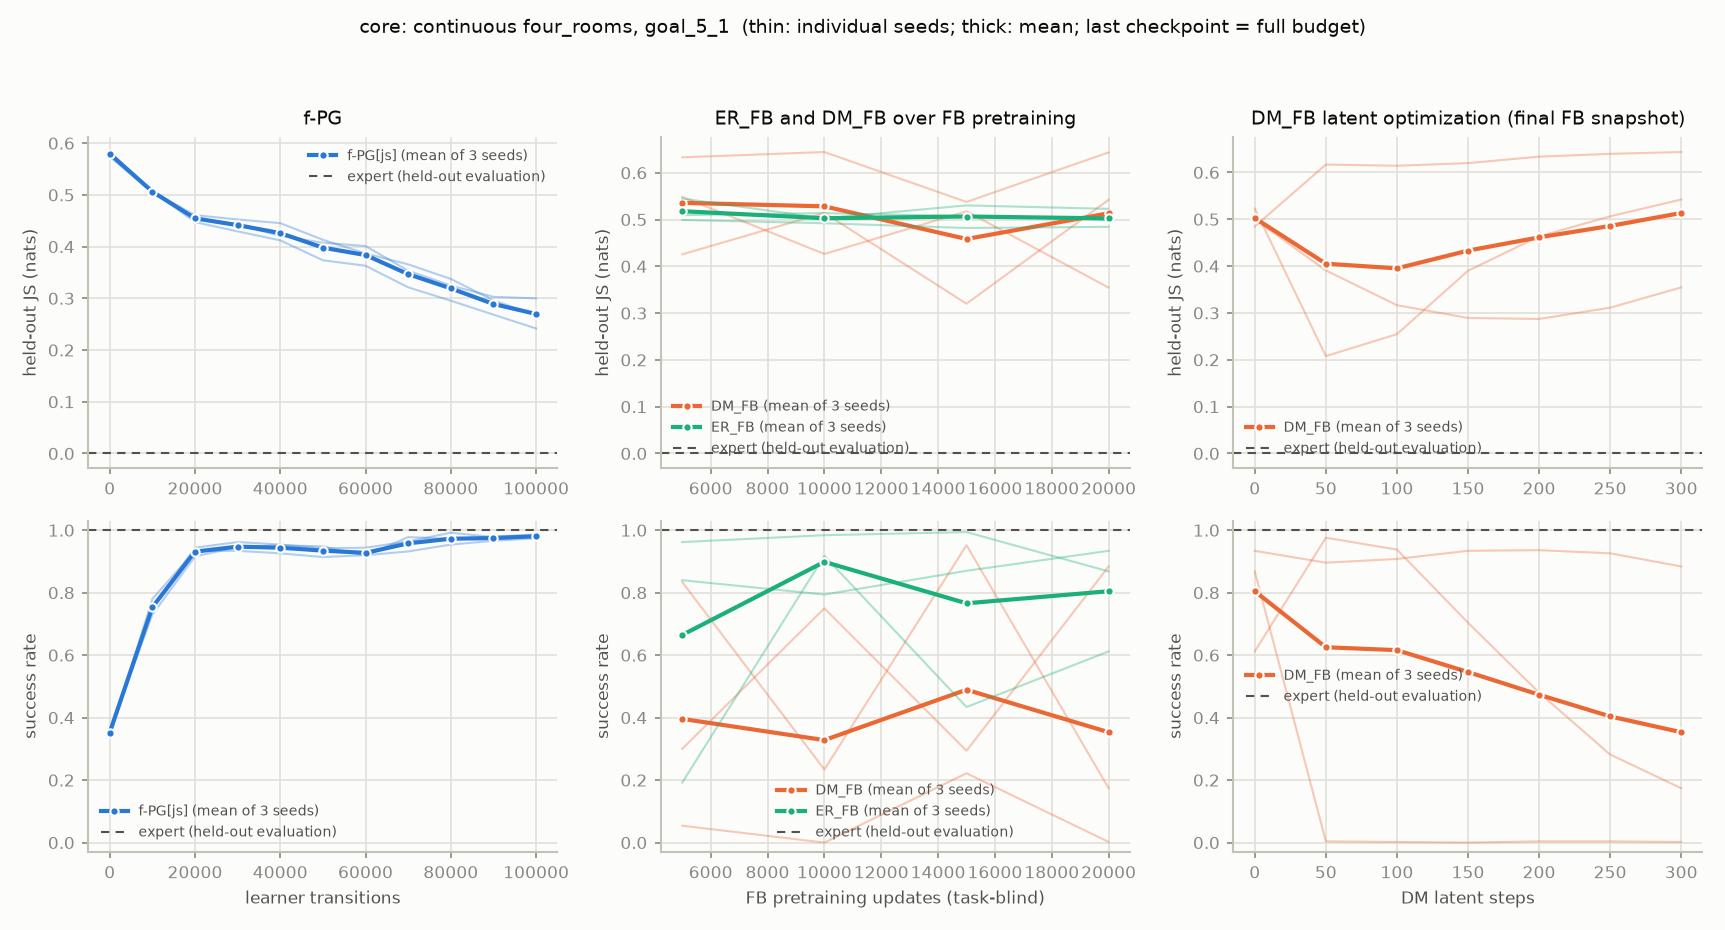
\includegraphics[width=\textwidth]{figures/curves_core_continuous_four_rooms_goal_5_1.png}
\caption{Learning curves, core suite, continuous four-rooms maze, goal (5,1).}
\end{figure}

\begin{figure}[p]
\centering
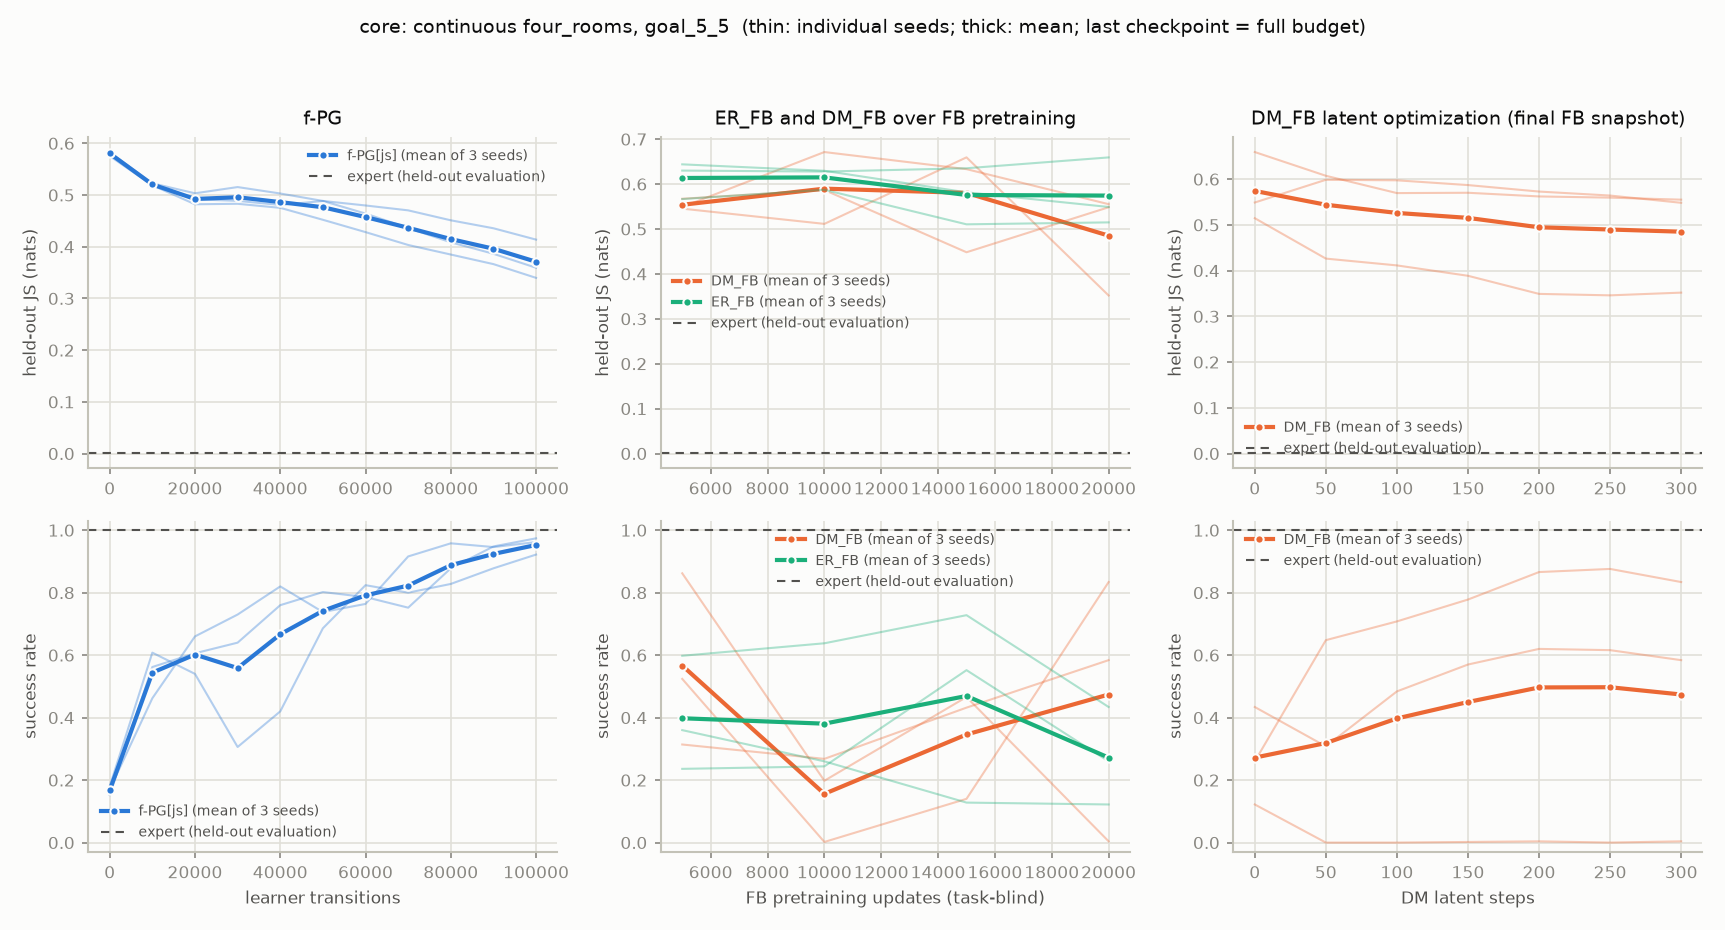
\includegraphics[width=\textwidth]{figures/curves_core_continuous_four_rooms_goal_5_5.png}
\caption{Learning curves, core suite, continuous four-rooms maze, goal (5,5).}
\end{figure}

\begin{figure}[p]
\centering
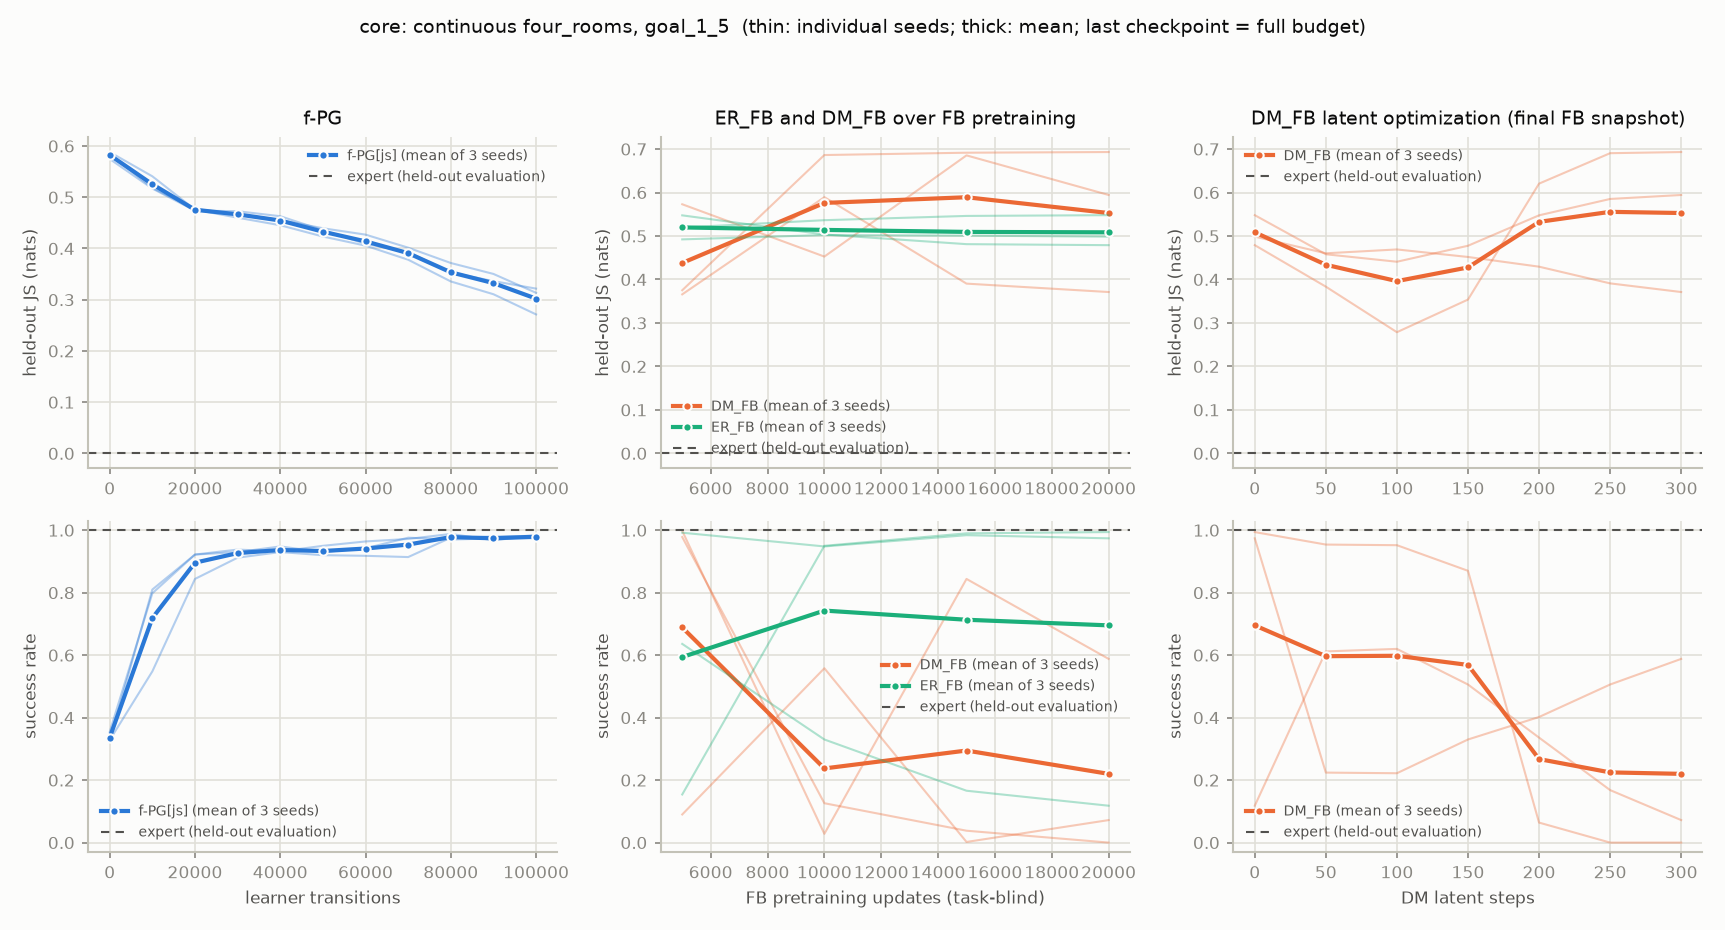
\includegraphics[width=\textwidth]{figures/curves_core_continuous_four_rooms_goal_1_5.png}
\caption{Learning curves, core suite, continuous four-rooms maze, goal (1,5).}
\end{figure}

\begin{figure}[p]
\centering
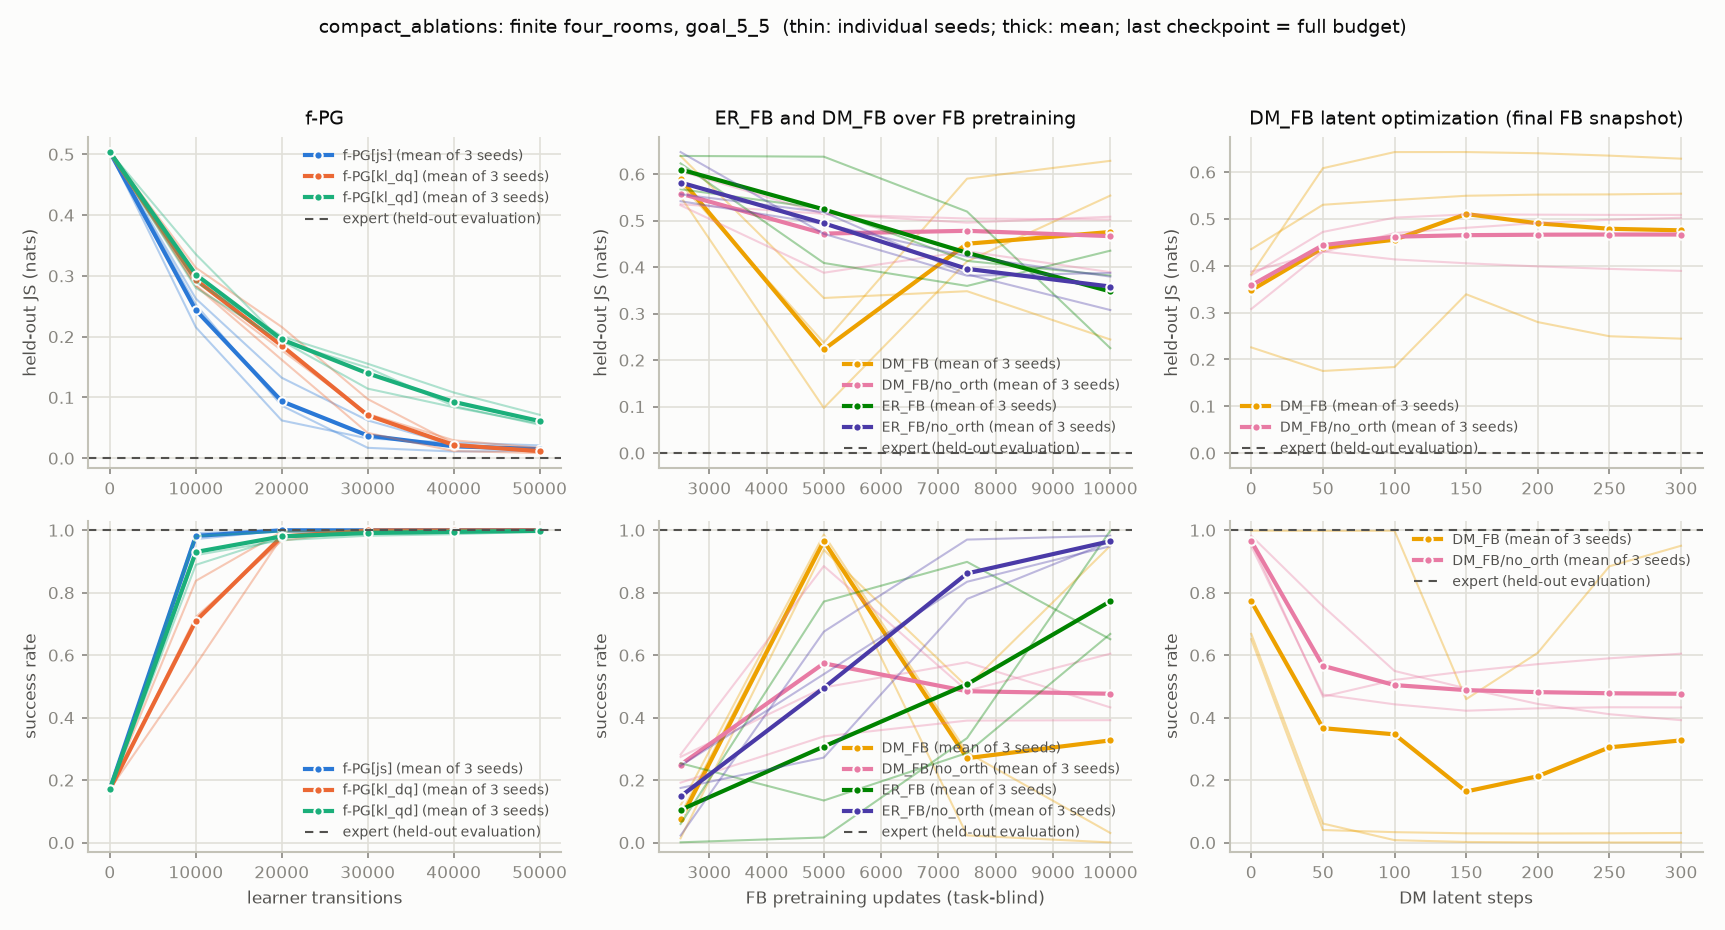
\includegraphics[width=\textwidth]{figures/curves_compact_ablations_finite_four_rooms_goal_5_5.png}\\[4pt]
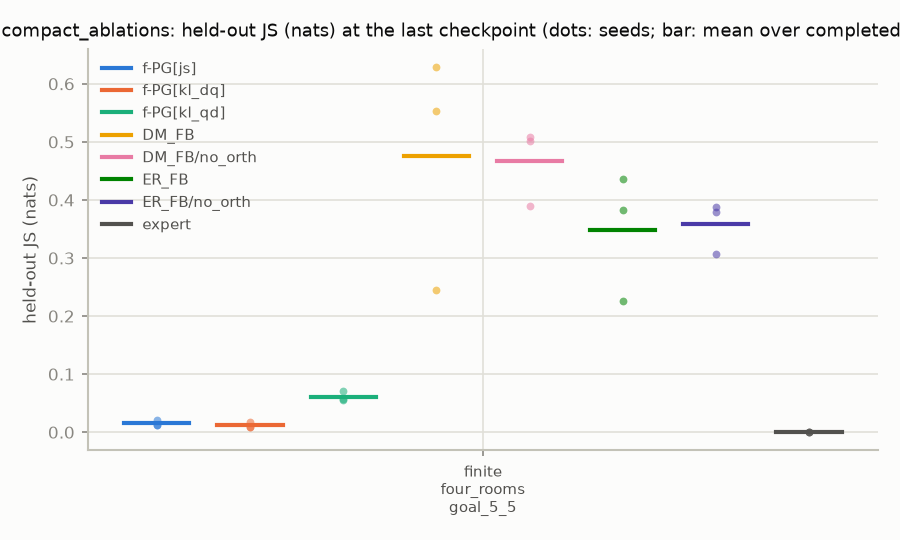
\includegraphics[width=0.49\textwidth]{figures/final_js_nats_compact_ablations.png}\hfill
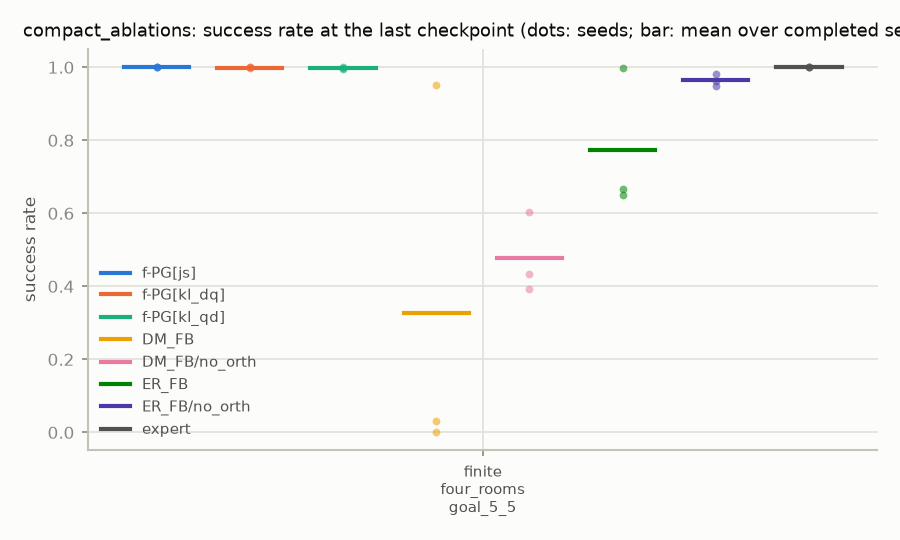
\includegraphics[width=0.49\textwidth]{figures/final_success_compact_ablations.png}
\caption{Compact ablations (four rooms, goal $(5,5)$): learning curves of every variant (top) and the final divergence and success of each seed (bottom).}\label{fig:curves-ablation}
\end{figure}
\FloatBarrier
